
\section{Additional Figures from Simulations}
\begin{figure}[h]
\centering
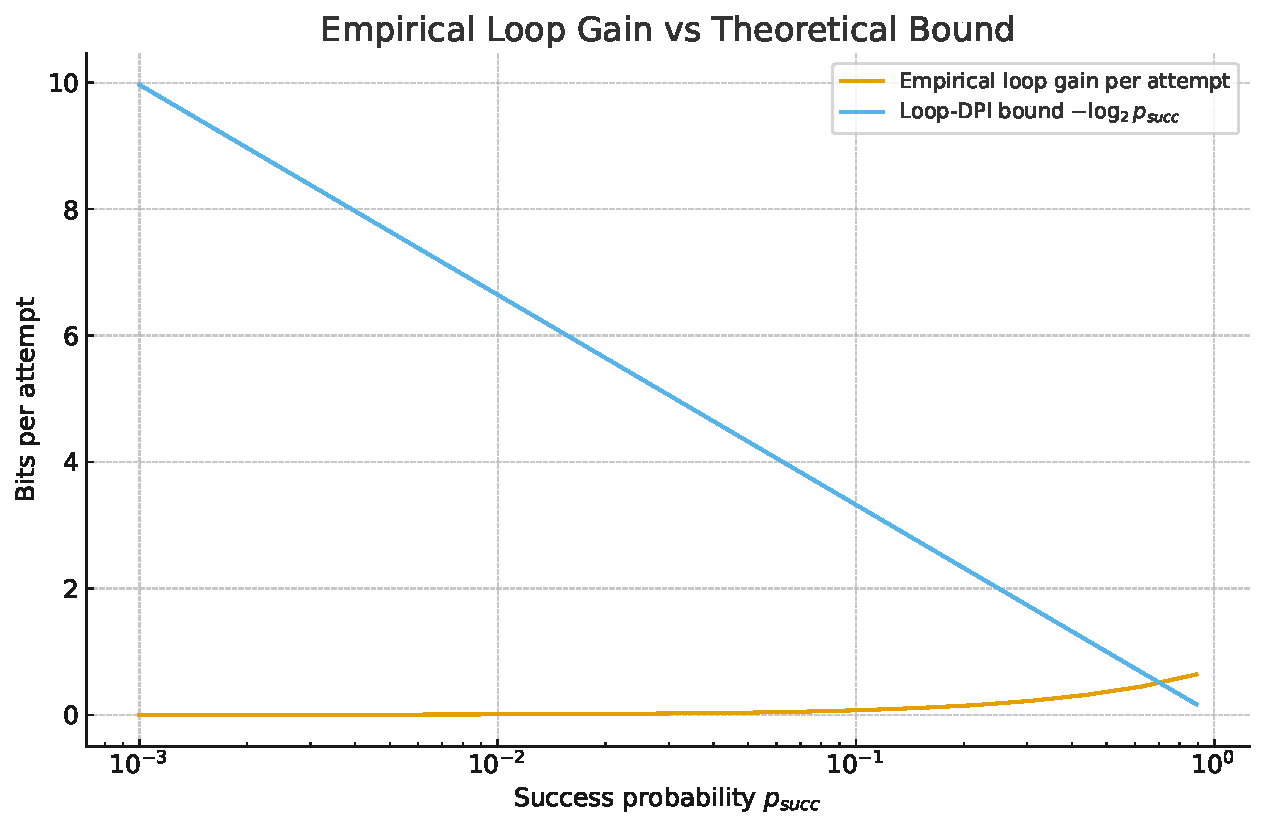
\includegraphics[width=0.7\linewidth]{figures/empirical_vs_bound.pdf}
\caption{Empirical loop information gain per attempt versus the Loop-DPI bound as a function of postselection success probability.}
\end{figure}

\begin{figure}[h]
\centering
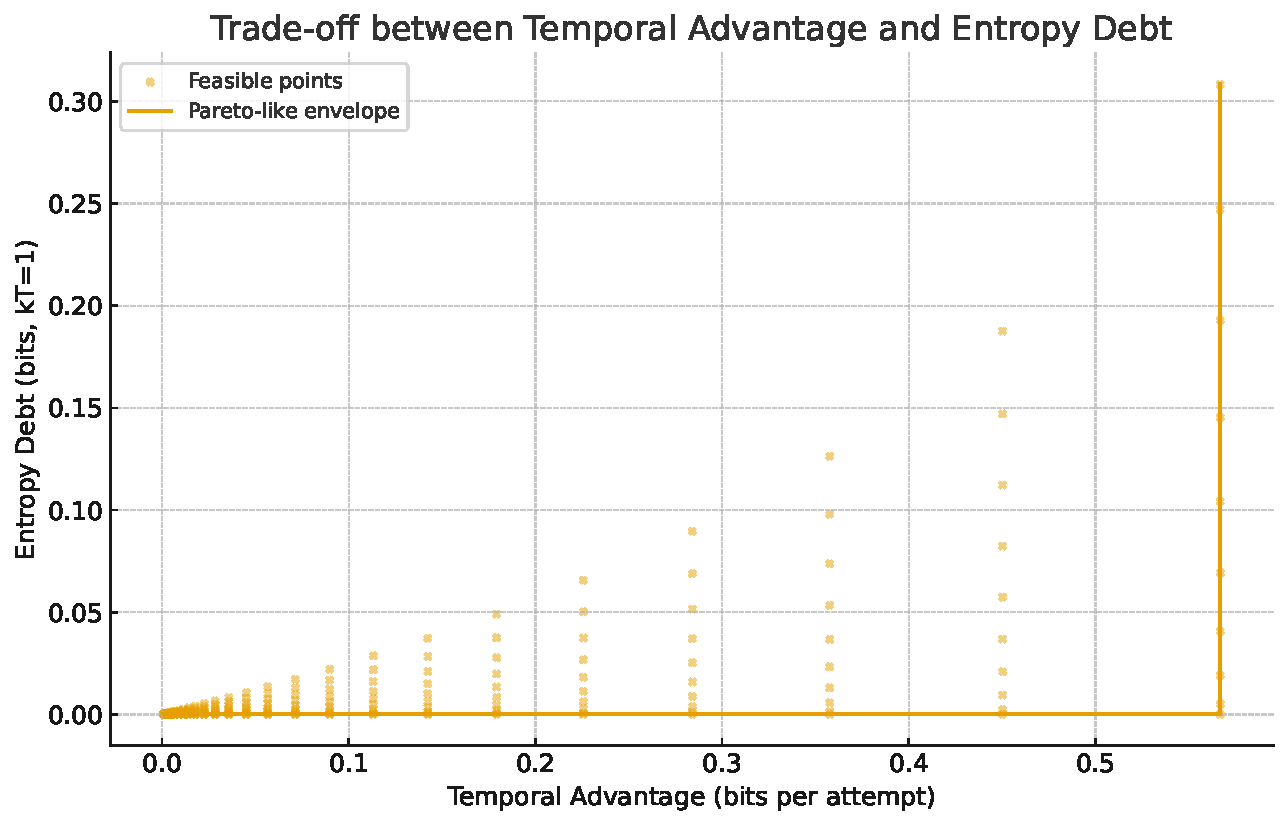
\includegraphics[width=0.7\linewidth]{figures/pareto_frontier.pdf}
\caption{Pareto-like trade-off between Temporal Advantage and Entropy Debt under varying success probabilities and paradox fractions.}
\end{figure}

\begin{figure}[h]
\centering
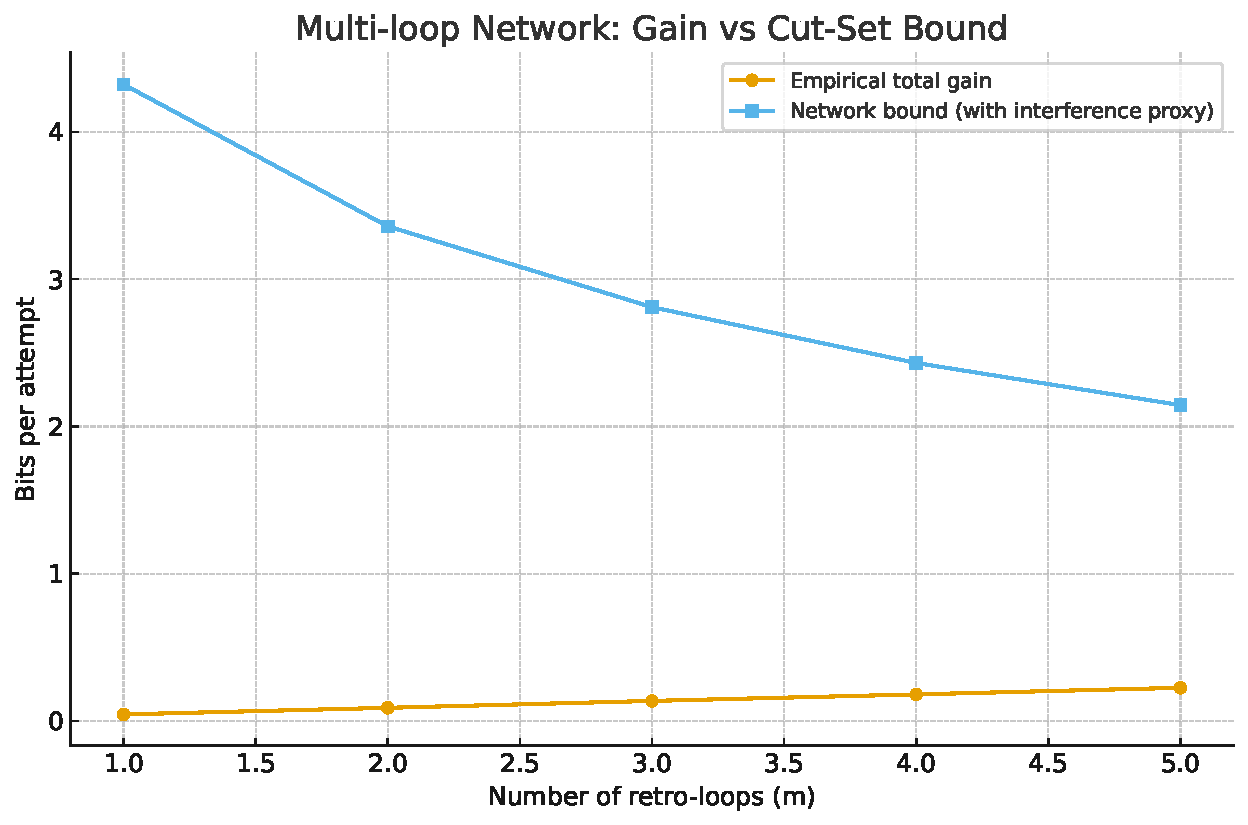
\includegraphics[width=0.7\linewidth]{figures/multiloop_gain.pdf}
\caption{Multi-loop network empirical gain compared with a cut-set style bound that includes an interference proxy.}
\end{figure}

\begin{figure}[h]
\centering
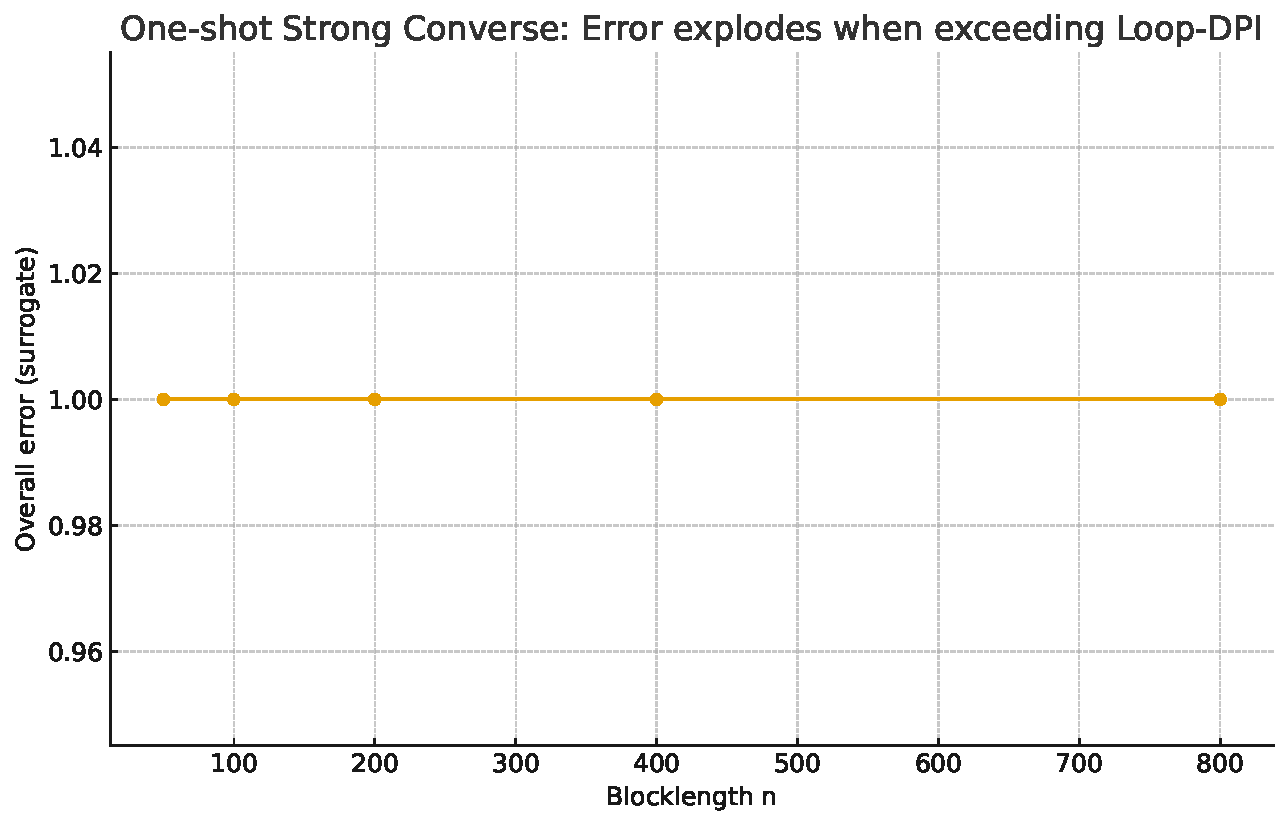
\includegraphics[width=0.7\linewidth]{figures/one_shot_converse.pdf}
\caption{Surrogate demonstration of the single-shot strong converse: attempting rates above the Loop-DPI bound drives error toward one with blocklength.}
\end{figure}


\begin{figure}[h]
\centering
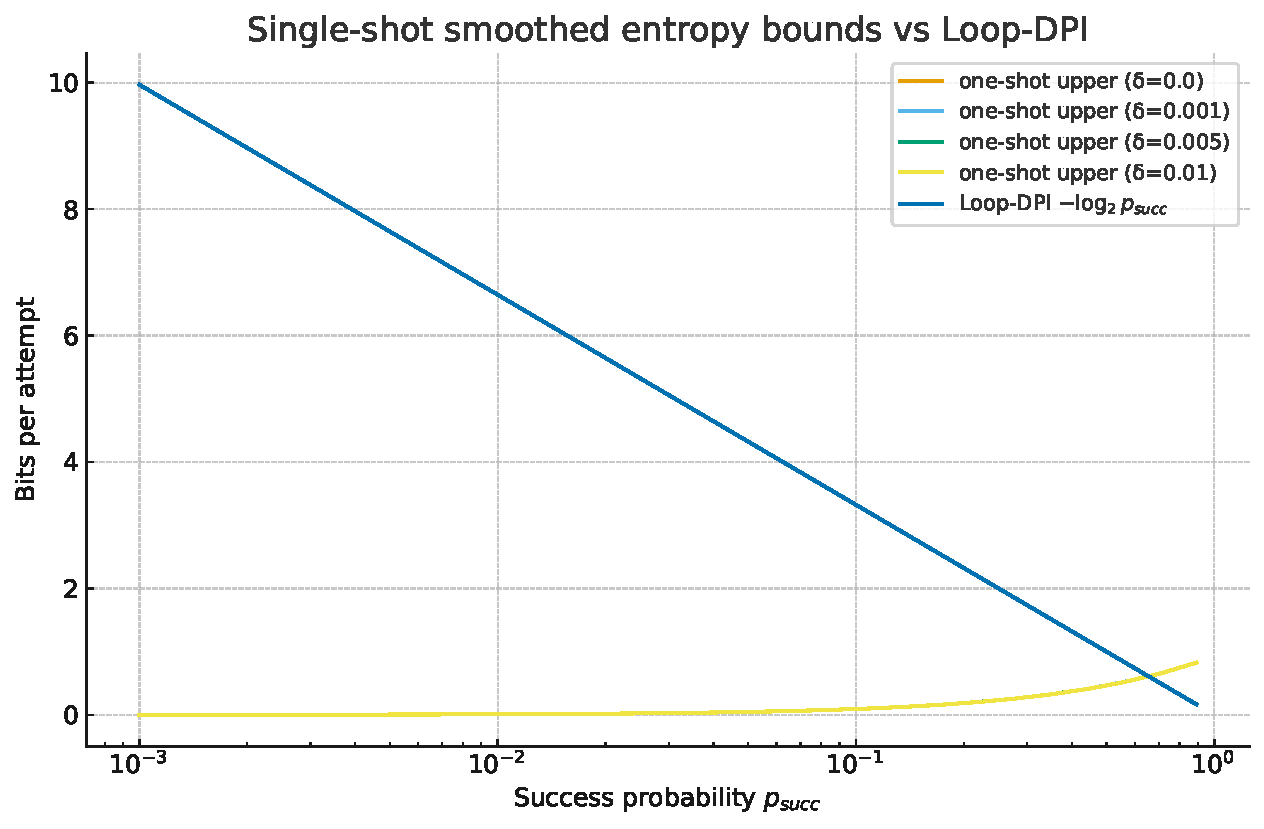
\includegraphics[width=0.7\linewidth]{figures/one_shot_smoothed.pdf}
\caption{Single-shot (smoothed entropy) upper bounds on achievable loop bits per attempt compared to the Loop-DPI asymptote.}
\end{figure}

\begin{figure}[h]
\centering
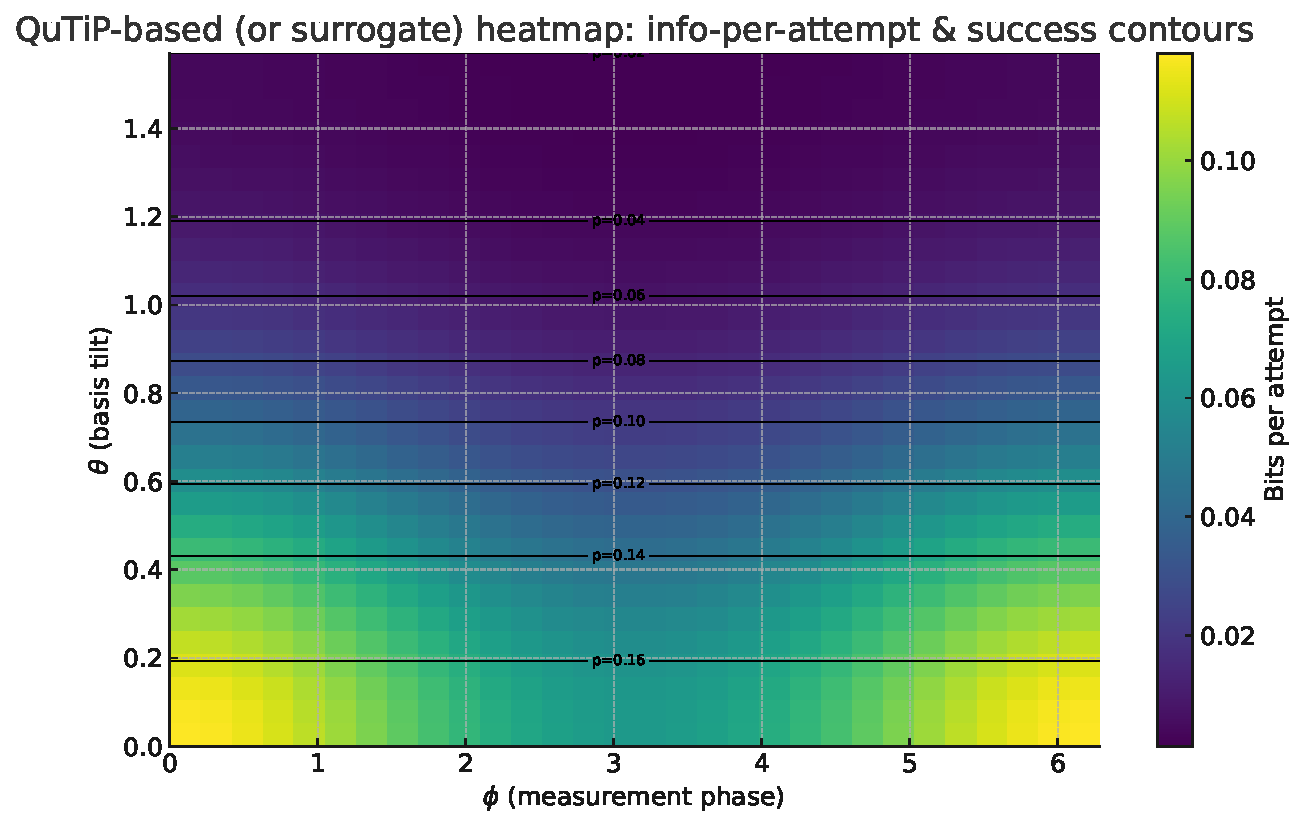
\includegraphics[width=0.75\linewidth]{figures/qutip_heatmap.pdf}
\caption{Heatmap of bits-per-attempt as a function of measurement basis $(\theta,\phi)$ with success-probability contours.}
\end{figure}
